\section{Self-sovereign data management}\label{solutions}
There are three customary methods of managing identifying data. The most common of which is the Isolated User Identity (SILO) Model \cite{federated}. Each service stores the required and requested user data, which the user can access when they authenticate with a username and password. This approach introduces two main drawbacks, which were both already mentioned before. First, there is a vast amount of data duplication that exists in different databases. Second, users are not in control of their own data and any service that stores it can decide what they wish to do with the data they store. They could choose to delete it, effectively erasing a part of the online identity of their user.

Federated identity removes some of the centralization that the SILO model introduces. Users can login to multiple services using one account, such as their Google or Facebook account. However, the user is still not in control of their own data. As several services can make use of the same database, it does remove part of the data duplication problem. Furthermore, it is also simpler for users to control their data as there is a central overview of services that have access to their account. Still, the federated data management model is not a suitable solution in the end. The federation manages and stores the data, so a breach in their databases compromises the data of many users and many services. On top of that, the federation could delete the one account that users identify themselves with on multiple services. This has an even larger impact than the situation where one service deletes an account in the SILO Model as it eliminates a significantly larger portion of the users online identity.

Self-sovereign identity does provide this full control over data to users. The main contributor to this control is the storage of data. Data is stored in a decentralized fashion, such as on a blockchain. Sensitive data that should not be visible to anyone is stored locally on the device of the user. The user is the only person with the right to grant or revoke access to their data. Self-sovereign identity provides full autonomy.

\begin{figure}[h]
\centering
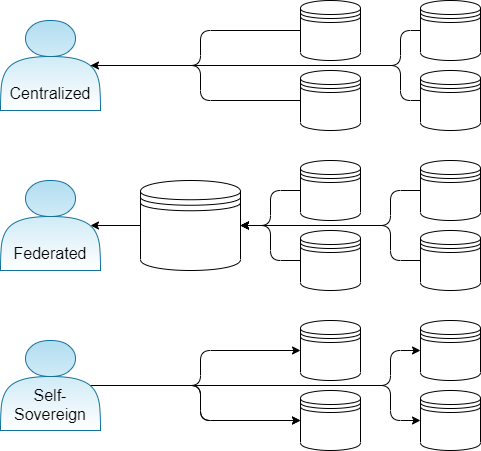
\includegraphics[scale=0.48]{figures/federated.png}
\vspace{-0.3cm}
\caption{The flow of data in the different management systems}
\label{fig:attestations}
\end{figure}

\subsection{Verifiable claims}
Verifiable claims (VCs) lie at the heart of SSI solutions. Almost all data is sent through these claims. The key idea is that the user will never have to send sensitive information. Rather, a claim is made, to which the user can answer. The service now has the information they require and the user did not send any sensitive data over a network.  

In the process of sending claims, three parties are involved. The first party is the subject. This is the user of an application and the person that needs to identify themselves. The main focus of SSI is that the subject is in full control over their data and identity, deciding which other parties gain or lose access. However, often data has to be verified or issued by a trusted party, the issuer. An example of an issuer is the government, because they can provide a proof of date of birth or the fact that the subject has a drivers license. These proofs are called attestations and can be revoked, for example when the drivers license expires and the subject does not get it renewed. The third party involved in the flow of data is the relying party. This party often is a service that requests the subject for identification by making a verifiable claim.

\begin{figure}[h]
\centering
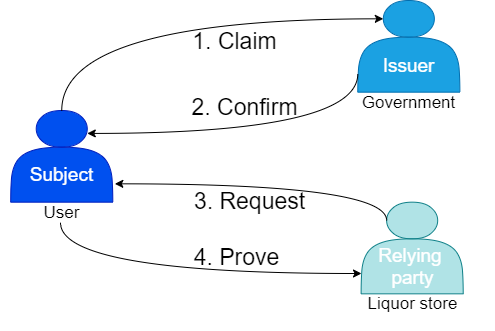
\includegraphics[scale=0.35]{figures/attestation.png}
\vspace{-0.3cm}
\caption{Parties involved in attesting data}
\label{fig:attestations}
\end{figure}

Upon receiving such a verifiable claim, the subject does not have to send the data to prove the claim. The VC acts as a polar question to which the subject can provide an answer. Instead of providing the subject's date of birth to verify they are over eighteen, they provide the signature of the government that was used to sign the attestation. These signatures are combined with some metadata to ensure they can only be used on this particular data. This metadata can, among others, contain a name, expiration date and signature scheme \cite{survey}.

Only forwarding these attestations has the advantage that no actual data about the user is sent over a network. If a malicious user were to get hold of the data they would not get any information about the subject. To ensure anonymity of users, it is paramount to send as little information as possible. The more is known about a user, the less anonymous they are.

\subsection{Limited autonomy}
The drawback of verifiable claims is that they are limited in the amount of data they are able to contain. Using only a polar question does not allow for any additional data to be sent. This implies that VCs alone will not be sufficient if SSI aims to replace all centralized services. Those services store more data about a user than can be requested through a verifiable claim. Almost every service that requires users to register with an account, stores the name of a user. This results in a great amount of duplication of stored data. However, it is hard, if not impossible, to make a verifiable claim about the name of a user when that name is not known to the service.

In many SSI solutions, this is solved by using an identifier for a user. The SSI solution \textcolor{red}{Blockstack [https://docs.stacks.co/build-apps/guides/data-storage]} stores public key identifiers on the blockchain and offers off-chain storage for other data. For the off-chain database, several cloud-computing applications are used, such as Dropbox and Google Drive. The advantage of this is that they are very fast in comparison with a blockchain. With this approach, it is a client-side responsibility to ensure data is properly formatted and encrypted if need be. This way, a service can request access to the data they need, without storing it locally. 

However, requesting that data requires more communication than is feasible with VCs. Still, claim portability is a key step towards full data portability, so this research will represent a universal architecture for the portability of verifiable claims. Further research could be conducted towards full data portability, as will be discussed in section \ref{further-research}.

